%% ----------------------------------------------------------------
%% AppendixA.tex
%% ---------------------------------------------------------------- 
\chapter{Listings} \label{Appendix:listing}

\begin{lstlisting}[caption=Code of the LSTM model's skeleton]
def normalize(vector):
    scaler = preprocessing.MinMaxScaler()
    return scaler.fit_transform(vector)

def sort_samples_by_link(data):
    sorted_data = {}
    for record in data:
        if record[0] in sorted_data.keys():
            sorted_data[record[0]].append(record[1:])
        else: sorted_data[record[0]] = [record[1:]]
    return sorted_data

def create_inout_sequences(data, shape):
    x = np.zeros((data.shape[0]-shape[0], shape[0], shape[1]))
    y = np.zeros((data.shape[0]-shape[0], 1))
    for i in range(data.shape[0]-shape[0]):
        train_seq = data[i:i+shape[0]]
        train_lbl = data[i+shape[0]:i+shape[0]+1][0][-1]
        x[i] = train_seq
        y[i] = train_lbl
    return x, y

ExpandedDataLoaded = sort_samples_by_link(load_expanded_data())
useData = np.array(ExpandedDataLoaded['4377906280329500514']) # Use one link

useData[:, 68] = normalize(useData[:, 68].reshape(-1, 1)).reshape(1, -1)
useData[:, 71:] = normalize(useData[:, 71:])

x, y = create_inout_sequences(useData, [30, 75])
X_train, X_test, y_train, y_test = train_test_split(x, y, test_size=0.1, 
                                                    shuffle=True)
model = Sequential()
earlystop = EarlyStopping(monitor='loss', min_delta=0, 
                            patience=3, verbose=1, restore_best_weights=True)
model.add(LSTM(units=140, return_sequences=False, 
                input_shape=(X_train.shape[1], X_train.shape[2])))
model.add(Dropout(0.2))
model.add(Dense(units=10, activation='sigmoid'))
model.compile(optimizer='adam', loss=tf.keras.losses.MeanSquaredError())
model.summary()

model.fit(X_train, y_train, epochs=100, batch_size=100, callbacks=earlystop)
\end{lstlisting}

\chapter{Charts} \label{Appendix:chart}

\begin{figure}[!htb]
    \centering
    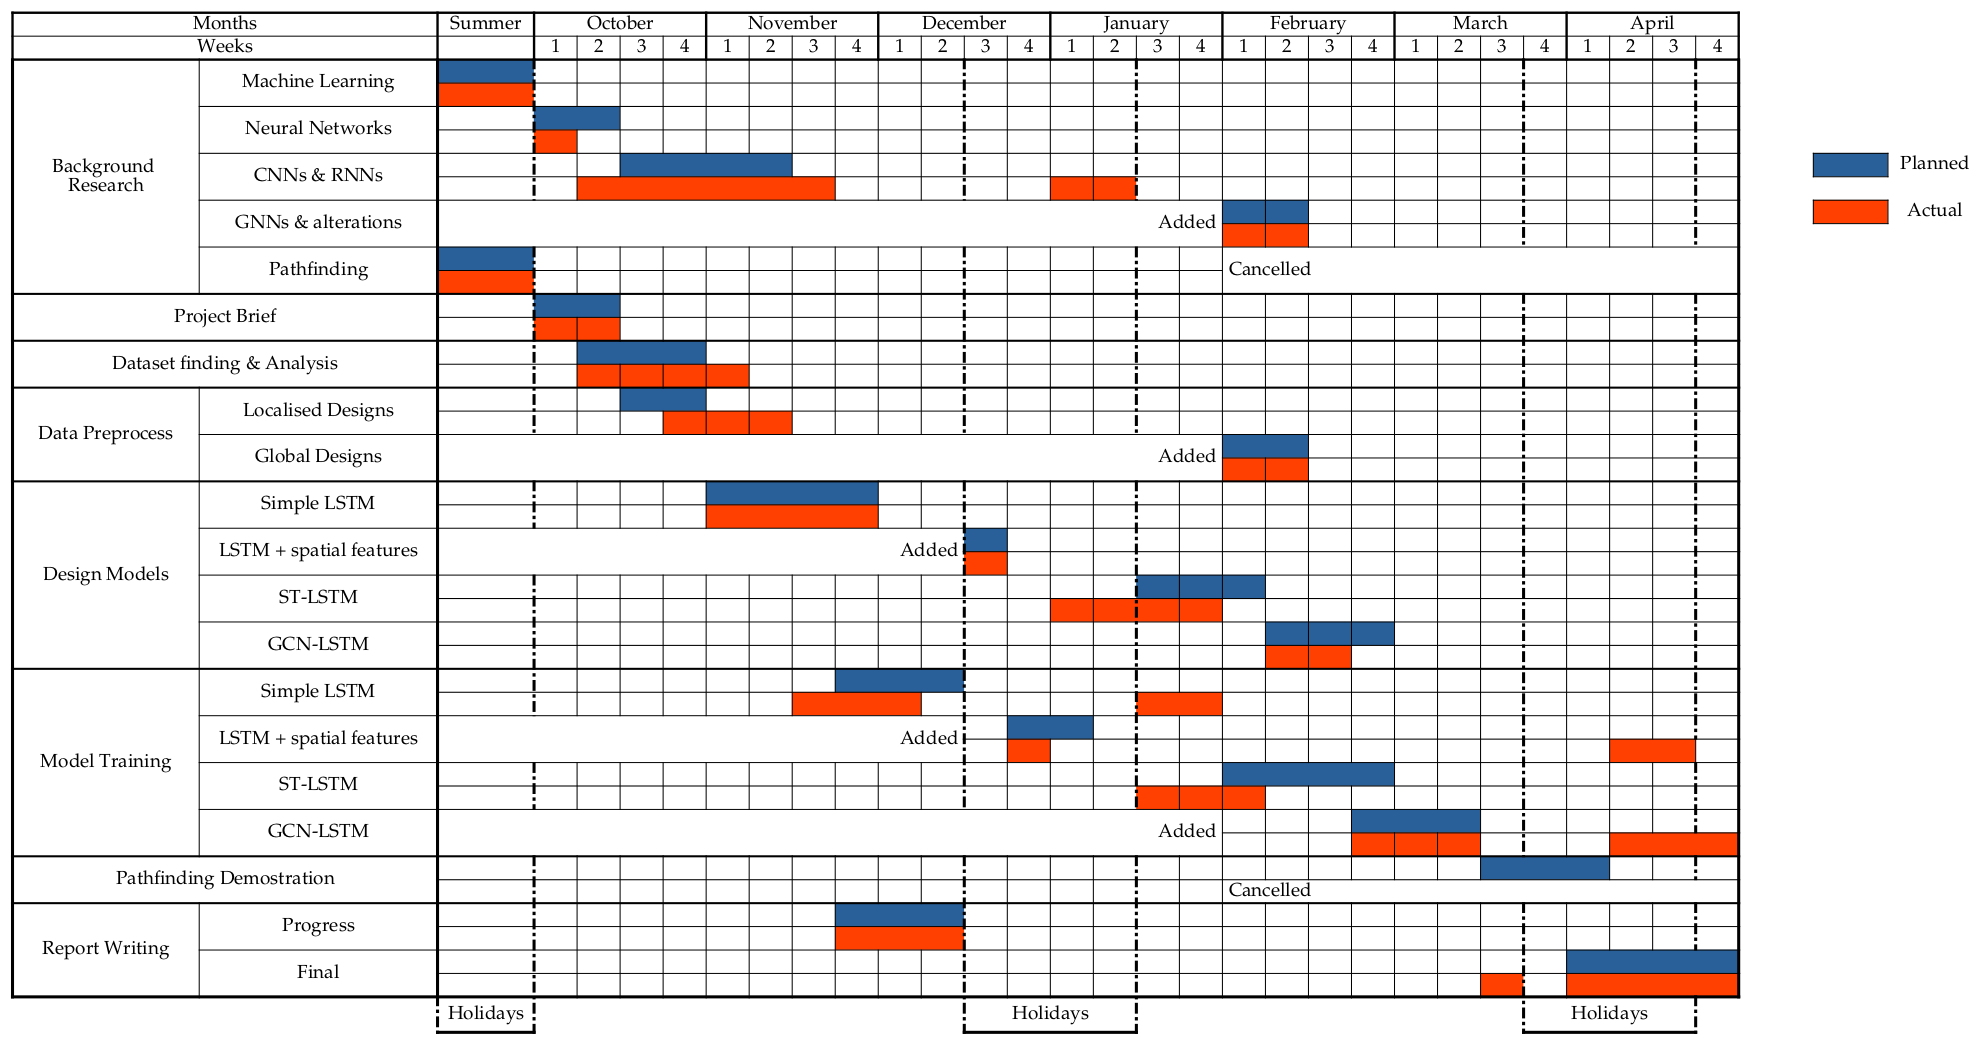
\includegraphics[width=7.8cm]{Gantt Chart}
    \caption{Gantt Chart}
    \label{Figure:gantt}
\end{figure}